\subsection{Auxiliary grids}

\begin{figure}
  \centering
  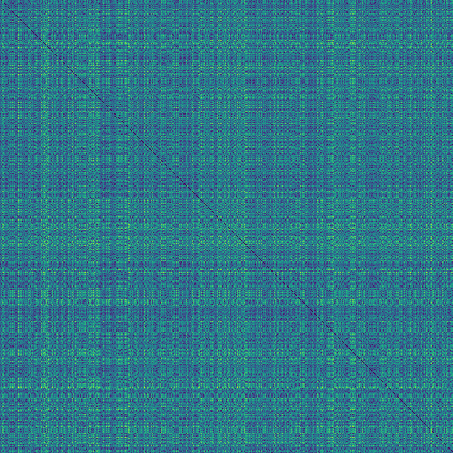
\includegraphics[width=0.4\textwidth]{figures/dist_mat_unsorted}
  \hspace{1cm}
  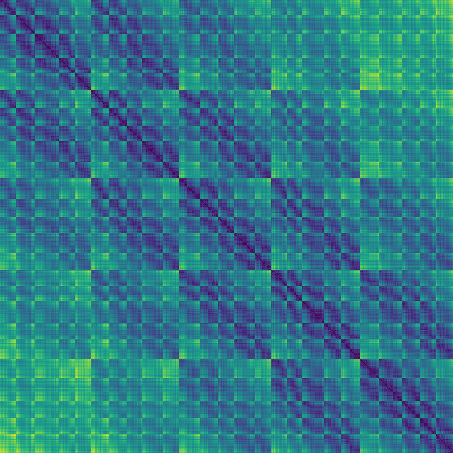
\includegraphics[width=0.4\textwidth]{figures/dist_mat_sorted}
  \caption{\label{fig:matrix structure} The interaction matrix for $g(\vb{r}, t) = \abs{\vb{r}}^{-1}$ between points randomly distributed throughout a unit cube appears to have very little structure (left).
    While we cannot fully order the points in three dimensions, we \emph{can} permute the matrix so as to give points within the same neighborhood adjacent indices.
    Points ordered thusly produce a diagonally-dominant interaction matrix with a hierarchical Toeplitz substructure (right).
    Such structures indicate portions of the matrix have very accurate low-rank approximations that offer the possibility of significant compression.
  }
\end{figure}

To effect a sub-quadratic calculation of \cref{eq:mot}, we approximate $\mathcal{G}^{(k)}$ as a sum of near- and far-field contributions.
The near-field matrix elements follow directly from \cref{eq:z elements}---sources within a prescribed distance threshold interact ``directly'' so as to avoid incurring unreasonable approximation error between adjacent basis functions.
Sources beyond this threshold, however, interact via auxiliary basis functions taken to reside at the vertices of a regular Cartesian grid.
These auxiliary sources recover $\mathfrak{F}\qty{g(\vb{r}, t) \ast \vb{P}(\vb{r}, t)}$ at large distances and impose a Toeplitz structure on the resulting interaction matrix.
This structure, then, lends itself to efficient $\mathcal{O}(N_s \log N_s)$ diagonalization through FFTs. 

\subsubsection{Potential evaluation: $g(\vb{r}, t) \ast \vb{P}(\vb{r}, t)$}

\begin{figure}
  \centering
  \usetikzlibrary{colorbrewer, decorations.pathreplacing, shapes}

\begin{tikzpicture}[>=latex, scale=2]
\draw[step=1, black, thick, opacity=0.1] (-2,-2) grid (3, 3);

\fill[cbblue, opacity=0.4] (0,0) rectangle (1, 1);
\fill[cbblue, opacity=0.2] (-1,-1) rectangle (2, 2);

\foreach \x in {-1,...,2} {
  \foreach \y in {-1,...,2} {

    \draw[thick, cbblue, fill=white, radius=0.1] (\x,\y) circle;

  }
}


\fill[cbblue, radius=0.03] (0.2, 0.7) node (A) {} circle;
\fill[cbblue, radius=0.03] (0.5, 0.2) node (B) {} circle;
\fill[cbblue, radius=0.03] (0.8, 0.5) node (C) {} circle;

\foreach \x in {0, 0.333, ..., 1} {
  \foreach \y in {0, 0.333, ..., 1} {
    %\draw[cbblue, fill=white] (\x,\y) circle (0.05);
    %\draw[] (\x,\y) node[cross, cbblue] {};
  }
}

\draw[diamond] (1.5, 1.5);

%\draw (0.5, 0.5) node[cross out] {} circle (0.2);

\fill[cbblue, radius=0.06] node[anchor=north east] (0, 0) {$\mathbf{r}_\text{box}$} circle;

\node[cbblue] (pts) at (0.5, 1.2) {Particles};
\draw[cbblue, ->] (pts) -- (A);
\draw[cbblue, ->] (pts) -- (B);
\draw[cbblue, ->] (pts) -- (C);

\draw[cbblue, thick, decorate,decoration={brace,amplitude=10}] (-1.1,2.2) -- (2.1, 2.2) node [midway, above, yshift=10] {Expansion region};
\draw[cbblue, thick, decorate,decoration={brace,amplitude=10}] (1.1,1.1) -- (1.1, -0.1) node [midway, right, xshift=10] {Box};

\draw[<->, cbblue] (-2, -1.8) -- (-1, -1.8) node [midway, fill=white] {$s_x$};
\draw[<->, cbblue] (-1.8, -2) -- (-1.8, -1) node [midway, fill=white] {$s_y$};

\end{tikzpicture}

  \caption{\label{fig:aim terminology} Illustration of the grid structure and terminology.
    All of the sources within a box (shown as the central shaded square) map to the same set of expansion points (shown as open circles) indexed relative to $\vb{r}_\text{box} = \floor{\vb{r}/s}$.
  }
\end{figure}

We represent the primary $\vb{s}_\ell(\vb{r})$ basis functions as a weighted sum of $\delta$-functions on the surrounding gridpoints , i.e.
\begin{equation}
  \psi_\ell(\vb{r}) \approx \sum_{\vb{u} \in B_{\ell}} \Lambda_{\ell\vb{u}} \delta(\vb{r} - \vb{u}).
  \label{eq:grid linear combination}
\end{equation}
Here, $\psi_\ell(\vb{r}) \in \qty{\vb{s}_\ell(\vb{r})\cdot \vu{x}, \vb{s}_\ell(\vb{r}) \cdot \vu{y}, \vb{s}_\ell(\vb{r}) \cdot \vu{z}}$ and $B_\ell$ denotes the collection of grid points, $\vb{u}$, within the expansion region of $\vb{s}_\ell(\vb{r})$ (\cref{fig:aim terminology}).
For an expansion of order\footnote{In principle, one could expand to different orders in different cartesian directions, though this involves considerably more bookkeeping for relatively little benefit. Thus, for convenience, we take ``the expansion order'' to mean the expansion order in every direction.} $m$, this sum contains $(m + 1)^3$ terms corresponding to the $(m + 1)^3$ grid points nearest to $\vb{s}_\ell(\vb{r})$.
Consequently, the $\Lambda_{\ell \vb{u}}$ matrices contain few nonzero elements and we have elected to use a moment-matching scheme to capture the $(m + 1)^3$ multipole moments of $\vb{s}_\ell(\vb{r})$ according to
\begin{equation}
  \sint (x - x_0)^{m_x}(y - y_0)^{m_y}(z - z_0)^{m_z} \qty[\psi_\ell(\vb{r}) - \sum_{\vb{u} \in c_\ell}\Lambda_{\ell\vb{u}}\delta(\vb{r} - \vb{u})] \dd[3]{\vb{r}} = 0.
  \label{eq:moment matching}
\end{equation}
In this expression, $0 \leqslant m_x, m_y, m_z \leqslant m$ and $\vb{r}_0 \equiv x_0 \vu{x} + y_0 \vu{y} + z_0\vu{z}$ denotes the origin about which we compute the multipoles.
To determine the $\Lambda_{\ell \vb{u}}$, we then solve the least-squares system
\begin{equation}
  \sum_{\vb{u} \in B_\ell} W_{\vb{m}\vb{u}}\Lambda_{\ell\vb{u}} = Q_{\ell\vb{m}}
  \label{eq:expansion matrix system}
\end{equation}
where
\begin{subequations}
  \begin{align}
    W_{\vb{m}\vb{u}} &= (u_x - x_0)^{m_x} (u_y - y_0)^{m_y} (u_z - z_0)^{m_z} \label{eq:w matrix} \\
    Q_{\ell \vb{m}} &= \int_{} \psi_\ell(\vb{r}) (x - x_0)^{m_x} (y - y_0)^{m_y} (z - z_0)^{m_z} \dd[3]{\vb{r}} \label{eq:q vector}.
  \end{align}
\end{subequations}
With infinite precision, the choice of $\vb{r}_0$ merely sets a reference point for the multipole coordinate system.
To minimize numerical issues, we choose $\vb{r}_0$ at the center of $\vb{s}_\ell(\vb{r})$.

Substituting \cref{eq:grid linear combination} into \cref{eq:propagator} and projecting onto $\psi_{\ell'}(\vb{r})$ gives
\begin{equation}
  \mathcal{G}_{\ell \ell'} = \siint \qty( \siint \psi_{\ell'}(\vb{r}) g(\vb{r} - \vb{r}', t - t') \psi_\ell(\vb{r}') \dd[1]{t'} \dd[3]{\vb{r}'} ) \dd[1]{t} \dd[3]{\vb{r}}
\end{equation}

\begin{figure}
  \centering
  \usetikzlibrary{colorbrewer, decorations.pathreplacing}
\begin{tikzpicture}
\draw[step=1, black, thick, opacity=0.1] (-7,-8) grid (8, 8);

\draw[thick, decorate,decoration={brace,amplitude=10}] (-2.95,-0.95) -- (-1.05, -0.95) node [midway, above, yshift=10] {$\Delta s$};
\draw[thick, decorate,decoration={brace,amplitude=10}] (-3.05,-2.95) -- (-3.05, -1.05) node [midway, anchor=east, xshift=-10] {$\Delta s$};

\draw[thick, decorate,decoration={brace,amplitude=10}] (1.95,2.05) -- (1.95,3.95) node [midway, anchor=east, xshift=-10] {$\Delta s$};
\draw[thick, decorate,decoration={brace,amplitude=10}] (2.05,4.05) -- (3.95,4.05) node [midway, anchor=south, yshift=10] {$\Delta s$};

\draw[thick, decorate,decoration={brace,amplitude=10}] (1.95,-3.95) -- (1.95,-1.05) node [midway, anchor=east, xshift=-10] {$\Delta s + 1$};
\draw[thick, decorate,decoration={brace,amplitude=10}] (3.95,-4.05) -- (2.05,-4.05) node [midway, anchor=north, yshift=-10] {$\Delta s$};

\fill[cbblue] (0,0) rectangle (1, 1);
\fill[cbblue, opacity=0.2] (-1,-1) rectangle (2, 2);

\foreach \x in {-1,...,2} {
  \foreach \y in {-1,...,2} {

    \draw[cbblue, fill=white, radius=0.1] (\x,\y) circle;

  }
}
\fill[cbblue, radius=0.06] node[anchor=north east] (0, 0) {$\mathbf{r}_0$} circle;




\fill[cbred] (-5,-5) rectangle (-4, -4);
\fill[cbred, opacity=0.2] (-6,-6) rectangle (-3, -3);

\foreach \x in {-6,-5,...,-3} {
  \foreach \y in {-6, -5, ..., -3} {
    \draw[cbred, fill=white, radius=0.1] (\x, \y) circle;
  }
}
\fill[cbred, radius=0.06] (-5, -5) node[anchor=north east, xshift=-3, yshift=-3] {$\mathbf{r}_a$} circle;




\fill[cbred] (5,5) rectangle (6, 6);
\fill[cbred, opacity=0.2] (4, 4) rectangle (7, 7);

\foreach \x in {4,...,7} {
  \foreach \y in {4,...,7} {
    \draw[cbred, fill=white, radius=0.1] (\x, \y) circle;
  }
}
\fill[cbred, radius=0.06] (5, 5) node[anchor=north east] {$\mathbf{r}_b$} circle;




\fill[cbgreen] (5,-6) rectangle (6, -5);
\fill[cbgreen, opacity=0.2] (4, -7) rectangle (7, -4);

\foreach \x in {4,...,7} {
  \foreach \y in {-7,...,-4} {
    \draw[cbgreen, fill=white, radius=0.1] (\x, \y) circle;
  }
}
\fill[cbgreen, radius=0.06] (5, -6) node[anchor=north east] {$\mathbf{r}_c$} circle;

\draw[thick, dashed] (-5.2,-5.2) rectangle (5.2, 5.2);

\end{tikzpicture}

  \caption{\label{fig:nearfield criterion}Illustration of the nearfield criterion for a third order expansion.
    The dashed line indicates the complete nearfield of the box associated with \textcolor{cbblue}{$\vb{r}_0$}---i.e. all boxes that have an expansion point within $\Delta s$ of the expansion around \textcolor{cbblue}{$\vb{r}_0$}.
  }
\end{figure}

\begin{figure}
  \centering
  \conditionalFigureInput{figures/expansion-grid}
  \caption{\label{fig:expansion grid}Spatial expansion pattern for $\vb{s}_\ell(\vb{r}) = \delta(\vb{r} - \vb{r}_\ell)$.
    An expansion of order $m$ requires $(m + 1)^3$ grid points.
    Moreover, increasing the expansion order incorporates new points in such a way as to keep $\vb{s}_\ell(\vb{r})$ as close to the center of the expansion region as possible.
  }
\end{figure}

\begin{figure}
  \centering
  \conditionalFigureInput{figures/nf_correction}
  \caption{\label{fig:nearfield correction}Illustration of nearfield corrections between close boxes.
    Expansions $A$ and $B$ overlap, but only box $B$ lies in the nearfield of box $C$.
    Consequently, we must track the $BC$ interaction (dashed line) independently of the FFT-based convolution so as to remove its high-error contribution to the total field.
  }
\end{figure}
